\documentclass[1p]{elsarticle_modified}
%\bibliographystyle{elsarticle-num}

%\usepackage[colorlinks]{hyperref}
%\usepackage{abbrmath_seonhwa} %\Abb, \Ascr, \Acal ,\Abf, \Afrak
\usepackage{amsfonts}
\usepackage{amssymb}
\usepackage{amsmath}
\usepackage{amsthm}
\usepackage{scalefnt}
\usepackage{amsbsy}
\usepackage{kotex}
\usepackage{caption}
\usepackage{subfig}
\usepackage{color}
\usepackage{graphicx}
\usepackage{xcolor} %% white, black, red, green, blue, cyan, magenta, yellow
\usepackage{float}
\usepackage{setspace}
\usepackage{hyperref}

\usepackage{tikz}
\usetikzlibrary{arrows}

\usepackage{multirow}
\usepackage{array} % fixed length table
\usepackage{hhline}

%%%%%%%%%%%%%%%%%%%%%
\makeatletter
\renewcommand*\env@matrix[1][\arraystretch]{%
	\edef\arraystretch{#1}%
	\hskip -\arraycolsep
	\let\@ifnextchar\new@ifnextchar
	\array{*\c@MaxMatrixCols c}}
\makeatother %https://tex.stackexchange.com/questions/14071/how-can-i-increase-the-line-spacing-in-a-matrix
%%%%%%%%%%%%%%%

\usepackage[normalem]{ulem}

\newcommand{\msout}[1]{\ifmmode\text{\sout{\ensuremath{#1}}}\else\sout{#1}\fi}
%SOURCE: \msout is \stkout macro in https://tex.stackexchange.com/questions/20609/strikeout-in-math-mode

\newcommand{\cancel}[1]{
	\ifmmode
	{\color{red}\msout{#1}}
	\else
	{\color{red}\sout{#1}}
	\fi
}

\newcommand{\add}[1]{
	{\color{blue}\uwave{#1}}
}

\newcommand{\replace}[2]{
	\ifmmode
	{\color{red}\msout{#1}}{\color{blue}\uwave{#2}}
	\else
	{\color{red}\sout{#1}}{\color{blue}\uwave{#2}}
	\fi
}

\newcommand{\Sol}{\mathcal{S}} %segment
\newcommand{\D}{D} %diagram
\newcommand{\A}{\mathcal{A}} %arc


%%%%%%%%%%%%%%%%%%%%%%%%%%%%%5 test

\def\sl{\operatorname{\textup{SL}}(2,\Cbb)}
\def\psl{\operatorname{\textup{PSL}}(2,\Cbb)}
\def\quan{\mkern 1mu \triangleright \mkern 1mu}

\theoremstyle{definition}
\newtheorem{thm}{Theorem}[section]
\newtheorem{prop}[thm]{Proposition}
\newtheorem{lem}[thm]{Lemma}
\newtheorem{ques}[thm]{Question}
\newtheorem{cor}[thm]{Corollary}
\newtheorem{defn}[thm]{Definition}
\newtheorem{exam}[thm]{Example}
\newtheorem{rmk}[thm]{Remark}
\newtheorem{alg}[thm]{Algorithm}

\newcommand{\I}{\sqrt{-1}}
\begin{document}

%\begin{frontmatter}
%
%\title{Boundary parabolic representations of knots up to 8 crossings}
%
%%% Group authors per affiliation:
%\author{Yunhi Cho} 
%\address{Department of Mathematics, University of Seoul, Seoul, Korea}
%\ead{yhcho@uos.ac.kr}
%
%
%\author{Seonhwa Kim} %\fnref{s_kim}}
%\address{Center for Geometry and Physics, Institute for Basic Science, Pohang, 37673, Korea}
%\ead{ryeona17@ibs.re.kr}
%
%\author{Hyuk Kim}
%\address{Department of Mathematical Sciences, Seoul National University, Seoul 08826, Korea}
%\ead{hyukkim@snu.ac.kr}
%
%\author{Seokbeom Yoon}
%\address{Department of Mathematical Sciences, Seoul National University, Seoul, 08826,  Korea}
%\ead{sbyoon15@snu.ac.kr}
%
%\begin{abstract}
%We find all boundary parabolic representation of knots up to 8 crossings.
%
%\end{abstract}
%\begin{keyword}
%    \MSC[2010] 57M25 
%\end{keyword}
%
%\end{frontmatter}

%\linenumbers
%\tableofcontents
%
\newcommand\colored[1]{\textcolor{white}{\rule[-0.35ex]{0.8em}{1.4ex}}\kern-0.8em\color{red} #1}%
%\newcommand\colored[1]{\textcolor{white}{ #1}\kern-2.17ex	\textcolor{white}{ #1}\kern-1.81ex	\textcolor{white}{ #1}\kern-2.15ex\color{red}#1	}

{\Large $\underline{12a_{0681}~(K12a_{0681})}$}

\setlength{\tabcolsep}{10pt}
\renewcommand{\arraystretch}{1.6}
\vspace{1cm}\begin{tabular}{m{100pt}>{\centering\arraybackslash}m{274pt}}
\multirow{5}{120pt}{
	\centering
	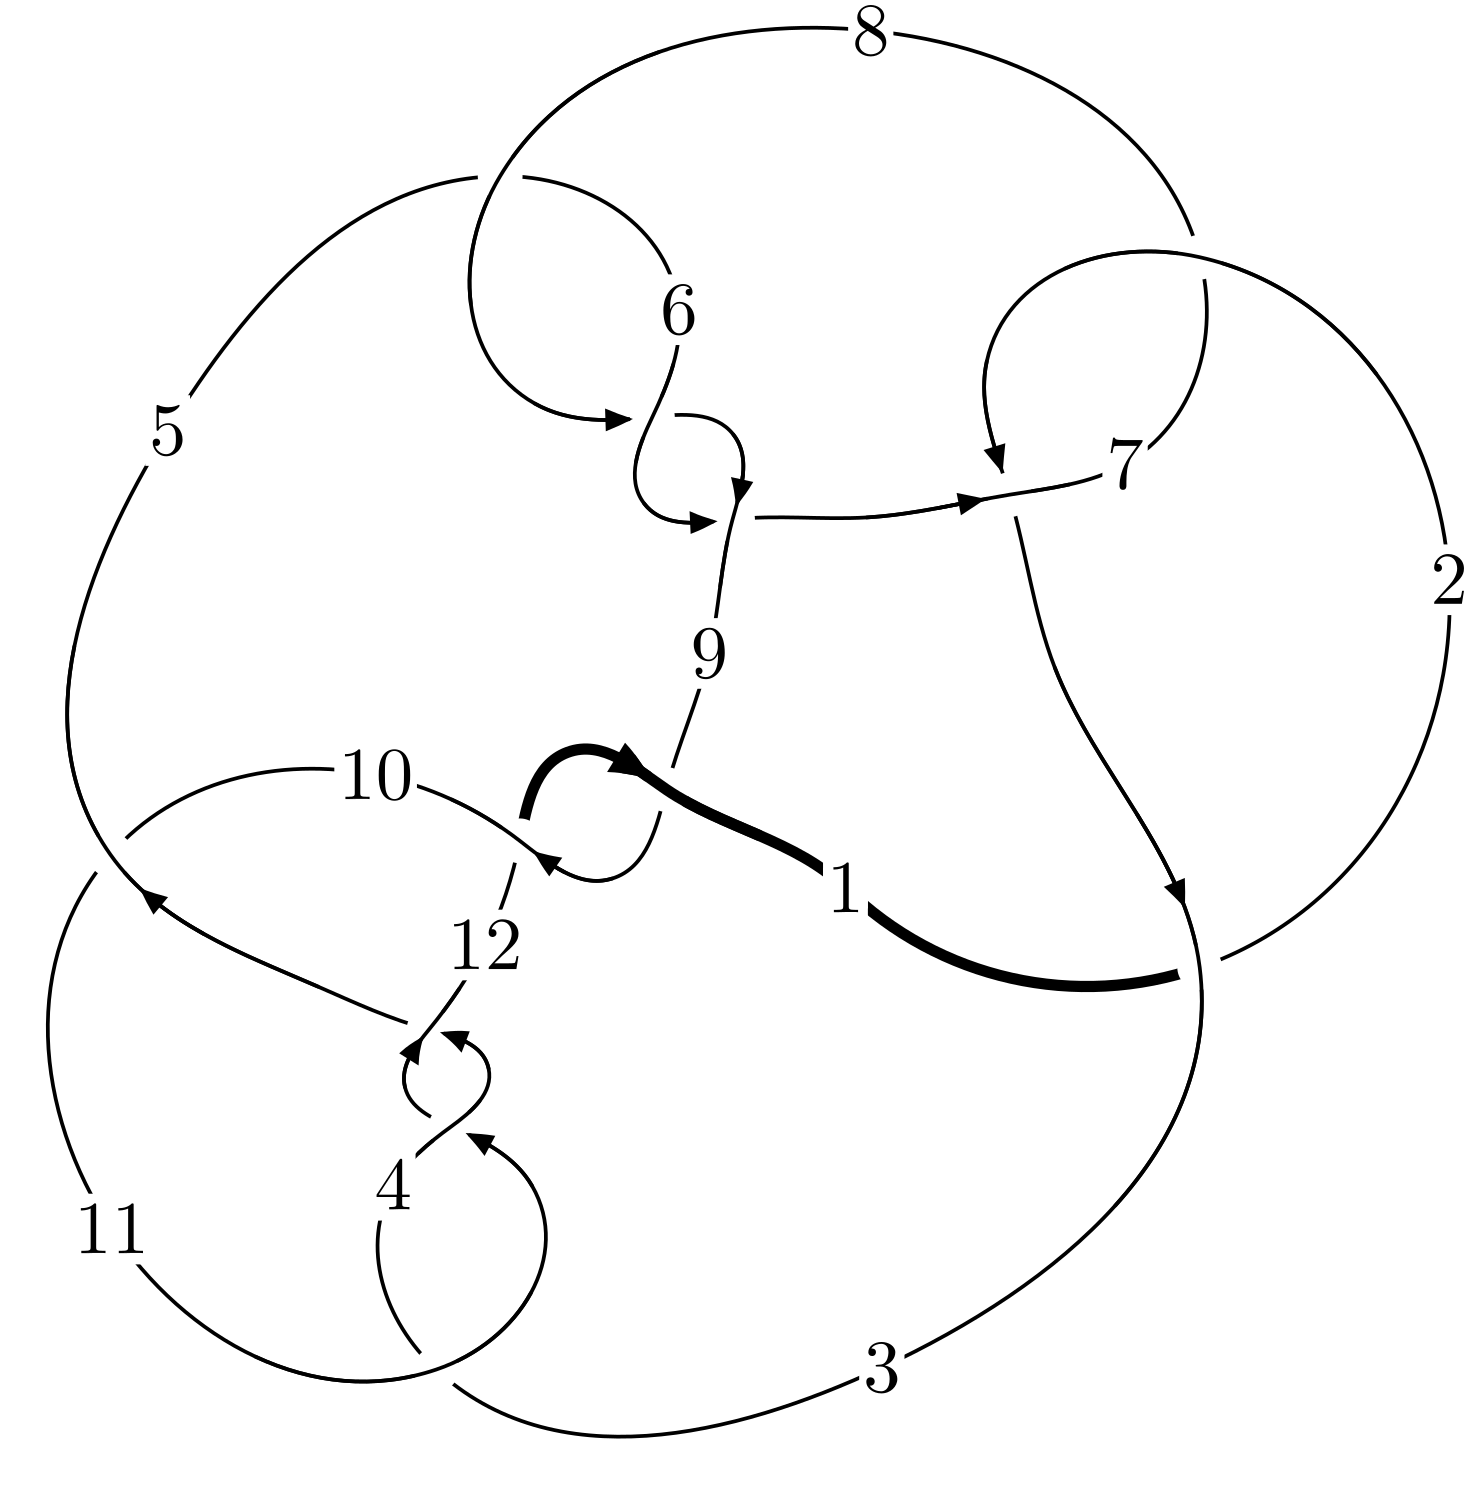
\includegraphics[width=112pt]{../../../GIT/diagram.site/Diagrams/png/1482_12a_0681.png}\\
\ \ \ A knot diagram\footnotemark}&
\allowdisplaybreaks
\textbf{Linearized knot diagam} \\
\cline{2-2}
 &
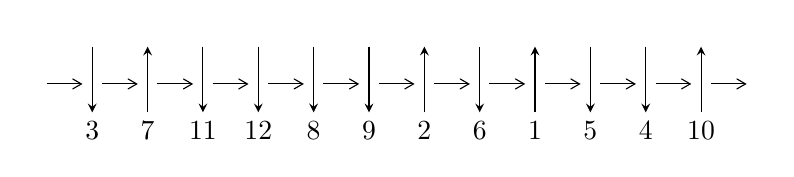
\begin{tikzpicture}[x=20pt, y=17pt]
	% nodes
	\node (C0) at (0, 0) {};
	\node (C1) at (1, 0) {};
	\node (C1U) at (1, +1) {};
	\node (C1D) at (1, -1) {3};

	\node (C2) at (2, 0) {};
	\node (C2U) at (2, +1) {};
	\node (C2D) at (2, -1) {7};

	\node (C3) at (3, 0) {};
	\node (C3U) at (3, +1) {};
	\node (C3D) at (3, -1) {11};

	\node (C4) at (4, 0) {};
	\node (C4U) at (4, +1) {};
	\node (C4D) at (4, -1) {12};

	\node (C5) at (5, 0) {};
	\node (C5U) at (5, +1) {};
	\node (C5D) at (5, -1) {8};

	\node (C6) at (6, 0) {};
	\node (C6U) at (6, +1) {};
	\node (C6D) at (6, -1) {9};

	\node (C7) at (7, 0) {};
	\node (C7U) at (7, +1) {};
	\node (C7D) at (7, -1) {2};

	\node (C8) at (8, 0) {};
	\node (C8U) at (8, +1) {};
	\node (C8D) at (8, -1) {6};

	\node (C9) at (9, 0) {};
	\node (C9U) at (9, +1) {};
	\node (C9D) at (9, -1) {1};

	\node (C10) at (10, 0) {};
	\node (C10U) at (10, +1) {};
	\node (C10D) at (10, -1) {5};

	\node (C11) at (11, 0) {};
	\node (C11U) at (11, +1) {};
	\node (C11D) at (11, -1) {4};

	\node (C12) at (12, 0) {};
	\node (C12U) at (12, +1) {};
	\node (C12D) at (12, -1) {10};
	\node (C13) at (13, 0) {};

	% arrows
	\draw[->,>={angle 60}]
	(C0) edge (C1) (C1) edge (C2) (C2) edge (C3) (C3) edge (C4) (C4) edge (C5) (C5) edge (C6) (C6) edge (C7) (C7) edge (C8) (C8) edge (C9) (C9) edge (C10) (C10) edge (C11) (C11) edge (C12) (C12) edge (C13) ;	\draw[->,>=stealth]
	(C1U) edge (C1D) (C2D) edge (C2U) (C3U) edge (C3D) (C4U) edge (C4D) (C5U) edge (C5D) (C6U) edge (C6D) (C7D) edge (C7U) (C8U) edge (C8D) (C9D) edge (C9U) (C10U) edge (C10D) (C11U) edge (C11D) (C12D) edge (C12U) ;
	\end{tikzpicture} \\
\hhline{~~} \\& 
\textbf{Solving Sequence} \\ \cline{2-2} 
 &
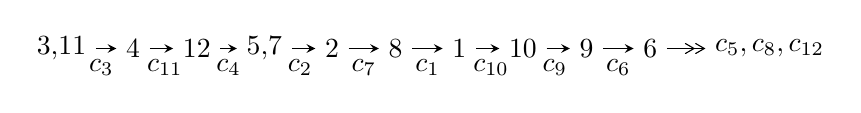
\begin{tikzpicture}[x=23pt, y=7pt]
	% node
	\node (A0) at (-1/8, 0) {3,11};
	\node (A1) at (1, 0) {4};
	\node (A2) at (2, 0) {12};
	\node (A3) at (49/16, 0) {5,7};
	\node (A4) at (33/8, 0) {2};
	\node (A5) at (41/8, 0) {8};
	\node (A6) at (49/8, 0) {1};
	\node (A7) at (57/8, 0) {10};
	\node (A8) at (65/8, 0) {9};
	\node (A9) at (73/8, 0) {6};
	\node (C1) at (1/2, -1) {$c_{3}$};
	\node (C2) at (3/2, -1) {$c_{11}$};
	\node (C3) at (5/2, -1) {$c_{4}$};
	\node (C4) at (29/8, -1) {$c_{2}$};
	\node (C5) at (37/8, -1) {$c_{7}$};
	\node (C6) at (45/8, -1) {$c_{1}$};
	\node (C7) at (53/8, -1) {$c_{10}$};
	\node (C8) at (61/8, -1) {$c_{9}$};
	\node (C9) at (69/8, -1) {$c_{6}$};
	\node (A10) at (11, 0) {$c_{5},c_{8},c_{12}$};

	% edge
	\draw[->,>=stealth]	
	(A0) edge (A1) (A1) edge (A2) (A2) edge (A3) (A3) edge (A4) (A4) edge (A5) (A5) edge (A6) (A6) edge (A7) (A7) edge (A8) (A8) edge (A9) ;
	\draw[->>,>={angle 60}]	
	(A9) edge (A10);
\end{tikzpicture} \\ 

\end{tabular} \\

\footnotetext{
The image of knot diagram is generated by the software ``\textbf{Draw programme}" developed by Andrew Bartholomew(\url{http://www.layer8.co.uk/maths/draw/index.htm\#Running-draw}), where we modified some parts for our purpose(\url{https://github.com/CATsTAILs/LinksPainter}).
}\phantom \\ \newline 
\centering \textbf{Ideals for irreducible components\footnotemark of $X_{\text{par}}$} 
 
\begin{align*}
I^u_{1}&=\langle 
u^{76}-35 u^{74}+\cdots+b-1,\;u^{75}+u^{74}+\cdots+a+1,\;u^{77}+2 u^{76}+\cdots- u-1\rangle \\
I^u_{2}&=\langle 
b,\;u^4- u^3- u^2+a+u,\;u^5- u^4-2 u^3+u^2+u+1\rangle \\
\\
\end{align*}
\raggedright * 2 irreducible components of $\dim_{\mathbb{C}}=0$, with total 82 representations.\\
\footnotetext{All coefficients of polynomials are rational numbers. But the coefficients are sometimes approximated in decimal forms when there is not enough margin.}
\newpage
\renewcommand{\arraystretch}{1}
\centering \section*{I. $I^u_{1}= \langle u^{76}-35 u^{74}+\cdots+b-1,\;u^{75}+u^{74}+\cdots+a+1,\;u^{77}+2 u^{76}+\cdots- u-1 \rangle$}
\flushleft \textbf{(i) Arc colorings}\\
\begin{tabular}{m{7pt} m{180pt} m{7pt} m{180pt} }
\flushright $a_{3}=$&$\begin{pmatrix}1\\0\end{pmatrix}$ \\
\flushright $a_{11}=$&$\begin{pmatrix}0\\u\end{pmatrix}$ \\
\flushright $a_{4}=$&$\begin{pmatrix}1\\u^2\end{pmatrix}$ \\
\flushright $a_{12}=$&$\begin{pmatrix}- u\\- u^3+u\end{pmatrix}$ \\
\flushright $a_{5}=$&$\begin{pmatrix}- u^2+1\\- u^4+2 u^2\end{pmatrix}$ \\
\flushright $a_{7}=$&$\begin{pmatrix}- u^{75}- u^{74}+\cdots-5 u-1\\- u^{76}+35 u^{74}+\cdots+u+1\end{pmatrix}$ \\
\flushright $a_{2}=$&$\begin{pmatrix}u^{11}-6 u^9+12 u^7-8 u^5+u^3-2 u\\- u^{11}+5 u^9-8 u^7+3 u^5+u^3+u\end{pmatrix}$ \\
\flushright $a_{8}=$&$\begin{pmatrix}- u^{75}- u^{74}+\cdots-10 u^2-4 u\\u^{76}-35 u^{74}+\cdots+9 u^2-1\end{pmatrix}$ \\
\flushright $a_{1}=$&$\begin{pmatrix}- u^9+4 u^7-5 u^5+2 u^3- u\\- u^{11}+5 u^9-8 u^7+3 u^5+u^3+u\end{pmatrix}$ \\
\flushright $a_{10}=$&$\begin{pmatrix}u^5-2 u^3+u\\u^7-3 u^5+2 u^3+u\end{pmatrix}$ \\
\flushright $a_{9}=$&$\begin{pmatrix}u^{13}-6 u^{11}+13 u^9-12 u^7+6 u^5-4 u^3+u\\u^{15}-7 u^{13}+18 u^{11}-19 u^9+6 u^7-2 u^5+4 u^3+u\end{pmatrix}$ \\
\flushright $a_{6}=$&$\begin{pmatrix}- u^{75}- u^{74}+\cdots-10 u^2-4 u\\u^{37}-17 u^{35}+\cdots+6 u^2+u\end{pmatrix}$\\&\end{tabular}
\flushleft \textbf{(ii) Obstruction class $= -1$}\\~\\
\flushleft \textbf{(iii) Cusp Shapes $= 2 u^{76}+4 u^{75}+\cdots-9 u-6$}\\~\\
\newpage\renewcommand{\arraystretch}{1}
\flushleft \textbf{(iv) u-Polynomials at the component}\newline \\
\begin{tabular}{m{50pt}|m{274pt}}
Crossings & \hspace{64pt}u-Polynomials at each crossing \\
\hline $$\begin{aligned}c_{1}\end{aligned}$$&$\begin{aligned}
&u^{77}+33 u^{76}+\cdots-7680 u-1024
\end{aligned}$\\
\hline $$\begin{aligned}c_{2},c_{7}\end{aligned}$$&$\begin{aligned}
&u^{77}+u^{76}+\cdots-96 u-32
\end{aligned}$\\
\hline $$\begin{aligned}c_{3},c_{4},c_{11}\end{aligned}$$&$\begin{aligned}
&u^{77}+2 u^{76}+\cdots- u-1
\end{aligned}$\\
\hline $$\begin{aligned}c_{5},c_{6},c_{8}\end{aligned}$$&$\begin{aligned}
&u^{77}-6 u^{76}+\cdots+u-1
\end{aligned}$\\
\hline $$\begin{aligned}c_{9},c_{12}\end{aligned}$$&$\begin{aligned}
&u^{77}+12 u^{76}+\cdots+1689 u+73
\end{aligned}$\\
\hline $$\begin{aligned}c_{10}\end{aligned}$$&$\begin{aligned}
&u^{77}-6 u^{76}+\cdots+813 u-935
\end{aligned}$\\
\hline
\end{tabular}\\~\\
\newpage\renewcommand{\arraystretch}{1}
\flushleft \textbf{(v) Riley Polynomials at the component}\newline \\
\begin{tabular}{m{50pt}|m{274pt}}
Crossings & \hspace{64pt}Riley Polynomials at each crossing \\
\hline $$\begin{aligned}c_{1}\end{aligned}$$&$\begin{aligned}
&y^{77}+13 y^{76}+\cdots+11141120 y-1048576
\end{aligned}$\\
\hline $$\begin{aligned}c_{2},c_{7}\end{aligned}$$&$\begin{aligned}
&y^{77}+33 y^{76}+\cdots-7680 y-1024
\end{aligned}$\\
\hline $$\begin{aligned}c_{3},c_{4},c_{11}\end{aligned}$$&$\begin{aligned}
&y^{77}-72 y^{76}+\cdots+7 y-1
\end{aligned}$\\
\hline $$\begin{aligned}c_{5},c_{6},c_{8}\end{aligned}$$&$\begin{aligned}
&y^{77}-68 y^{76}+\cdots-7 y-1
\end{aligned}$\\
\hline $$\begin{aligned}c_{9},c_{12}\end{aligned}$$&$\begin{aligned}
&y^{77}+60 y^{76}+\cdots+148363 y-5329
\end{aligned}$\\
\hline $$\begin{aligned}c_{10}\end{aligned}$$&$\begin{aligned}
&y^{77}-24 y^{76}+\cdots+24711039 y-874225
\end{aligned}$\\
\hline
\end{tabular}\\~\\
\newpage\flushleft \textbf{(vi) Complex Volumes and Cusp Shapes}
$$\begin{array}{c|c|c}  
\text{Solutions to }I^u_{1}& \I (\text{vol} + \sqrt{-1}CS) & \text{Cusp shape}\\
 \hline 
\begin{aligned}
u &= -1.118910 + 0.179695 I \\
a &= -0.440072 + 1.213090 I \\
b &= \phantom{-}0.513943 - 0.982821 I\end{aligned}
 & -4.41825 - 2.77630 I & \phantom{-0.000000 } 0 \\ \hline\begin{aligned}
u &= -1.118910 - 0.179695 I \\
a &= -0.440072 - 1.213090 I \\
b &= \phantom{-}0.513943 + 0.982821 I\end{aligned}
 & -4.41825 + 2.77630 I & \phantom{-0.000000 } 0 \\ \hline\begin{aligned}
u &= \phantom{-}0.388896 + 0.697285 I \\
a &= \phantom{-}2.58400 + 0.08701 I \\
b &= -0.694399 + 1.197770 I\end{aligned}
 & -6.76637 - 11.69120 I & -8.55592 + 8.80415 I \\ \hline\begin{aligned}
u &= \phantom{-}0.388896 - 0.697285 I \\
a &= \phantom{-}2.58400 - 0.08701 I \\
b &= -0.694399 - 1.197770 I\end{aligned}
 & -6.76637 + 11.69120 I & -8.55592 - 8.80415 I \\ \hline\begin{aligned}
u &= \phantom{-}0.467253 + 0.642938 I \\
a &= -1.072070 + 0.222088 I \\
b &= \phantom{-}0.025679 - 1.363990 I\end{aligned}
 & -11.71880 - 2.13120 I & -12.50690 + 3.22543 I \\ \hline\begin{aligned}
u &= \phantom{-}0.467253 - 0.642938 I \\
a &= -1.072070 - 0.222088 I \\
b &= \phantom{-}0.025679 + 1.363990 I\end{aligned}
 & -11.71880 + 2.13120 I & -12.50690 - 3.22543 I \\ \hline\begin{aligned}
u &= -1.199980 + 0.164041 I \\
a &= \phantom{-}0.765140 - 0.964895 I \\
b &= -0.662389 + 0.724093 I\end{aligned}
 & -0.198946 + 0.491194 I & \phantom{-0.000000 } 0 \\ \hline\begin{aligned}
u &= -1.199980 - 0.164041 I \\
a &= \phantom{-}0.765140 + 0.964895 I \\
b &= -0.662389 - 0.724093 I\end{aligned}
 & -0.198946 - 0.491194 I & \phantom{-0.000000 } 0 \\ \hline\begin{aligned}
u &= \phantom{-}0.550317 + 0.554367 I \\
a &= -0.557825 - 0.493865 I \\
b &= \phantom{-}0.660792 + 1.201360 I\end{aligned}
 & -7.39452 + 7.48341 I & -10.14800 - 2.91847 I \\ \hline\begin{aligned}
u &= \phantom{-}0.550317 - 0.554367 I \\
a &= -0.557825 + 0.493865 I \\
b &= \phantom{-}0.660792 - 1.201360 I\end{aligned}
 & -7.39452 - 7.48341 I & -10.14800 + 2.91847 I\\
 \hline 
 \end{array}$$\newpage$$\begin{array}{c|c|c}  
\text{Solutions to }I^u_{1}& \I (\text{vol} + \sqrt{-1}CS) & \text{Cusp shape}\\
 \hline 
\begin{aligned}
u &= \phantom{-}0.382467 + 0.674572 I \\
a &= -2.43549 - 0.42583 I \\
b &= \phantom{-}0.583029 - 1.060690 I\end{aligned}
 & -1.41933 - 7.47214 I & -5.05697 + 8.34642 I \\ \hline\begin{aligned}
u &= \phantom{-}0.382467 - 0.674572 I \\
a &= -2.43549 + 0.42583 I \\
b &= \phantom{-}0.583029 + 1.060690 I\end{aligned}
 & -1.41933 + 7.47214 I & -5.05697 - 8.34642 I \\ \hline\begin{aligned}
u &= -0.391946 + 0.660763 I \\
a &= \phantom{-}1.07868 - 1.47152 I \\
b &= -1.058370 + 0.462731 I\end{aligned}
 & -4.41478 + 5.37995 I & -7.77105 - 5.68914 I \\ \hline\begin{aligned}
u &= -0.391946 - 0.660763 I \\
a &= \phantom{-}1.07868 + 1.47152 I \\
b &= -1.058370 - 0.462731 I\end{aligned}
 & -4.41478 - 5.37995 I & -7.77105 + 5.68914 I \\ \hline\begin{aligned}
u &= \phantom{-}0.392387 + 0.638561 I \\
a &= \phantom{-}1.89360 + 0.81444 I \\
b &= -0.337099 + 0.970309 I\end{aligned}
 & -3.46473 - 2.75353 I & -9.00366 + 4.34907 I \\ \hline\begin{aligned}
u &= \phantom{-}0.392387 - 0.638561 I \\
a &= \phantom{-}1.89360 - 0.81444 I \\
b &= -0.337099 - 0.970309 I\end{aligned}
 & -3.46473 + 2.75353 I & -9.00366 - 4.34907 I \\ \hline\begin{aligned}
u &= -1.25296\phantom{ +0.000000I} \\
a &= -0.489598\phantom{ +0.000000I} \\
b &= \phantom{-}0.440012\phantom{ +0.000000I}\end{aligned}
 & -2.70327\phantom{ +0.000000I} & \phantom{-0.000000 } 0 \\ \hline\begin{aligned}
u &= \phantom{-}1.247280 + 0.146275 I \\
a &= -2.07717 - 0.81765 I \\
b &= \phantom{-}0.556055 - 0.712579 I\end{aligned}
 & -3.52703 - 1.49966 I & \phantom{-0.000000 } 0 \\ \hline\begin{aligned}
u &= \phantom{-}1.247280 - 0.146275 I \\
a &= -2.07717 + 0.81765 I \\
b &= \phantom{-}0.556055 + 0.712579 I\end{aligned}
 & -3.52703 + 1.49966 I & \phantom{-0.000000 } 0 \\ \hline\begin{aligned}
u &= \phantom{-}0.512426 + 0.536307 I \\
a &= \phantom{-}0.551321 + 0.026348 I \\
b &= -0.538012 - 1.042190 I\end{aligned}
 & -1.97887 + 3.43479 I & -6.68994 - 2.31052 I\\
 \hline 
 \end{array}$$\newpage$$\begin{array}{c|c|c}  
\text{Solutions to }I^u_{1}& \I (\text{vol} + \sqrt{-1}CS) & \text{Cusp shape}\\
 \hline 
\begin{aligned}
u &= \phantom{-}0.512426 - 0.536307 I \\
a &= \phantom{-}0.551321 - 0.026348 I \\
b &= -0.538012 + 1.042190 I\end{aligned}
 & -1.97887 - 3.43479 I & -6.68994 + 2.31052 I \\ \hline\begin{aligned}
u &= -0.488346 + 0.553137 I \\
a &= -1.48960 + 0.38906 I \\
b &= \phantom{-}1.044170 + 0.400052 I\end{aligned}
 & -4.84664 - 1.37205 I & -9.12609 - 0.79115 I \\ \hline\begin{aligned}
u &= -0.488346 - 0.553137 I \\
a &= -1.48960 - 0.38906 I \\
b &= \phantom{-}1.044170 - 0.400052 I\end{aligned}
 & -4.84664 + 1.37205 I & -9.12609 + 0.79115 I \\ \hline\begin{aligned}
u &= \phantom{-}1.254630 + 0.207259 I \\
a &= \phantom{-}2.05786 + 0.27148 I \\
b &= -0.637359 + 0.904548 I\end{aligned}
 & -0.73681 - 5.52218 I & \phantom{-0.000000 } 0 \\ \hline\begin{aligned}
u &= \phantom{-}1.254630 - 0.207259 I \\
a &= \phantom{-}2.05786 - 0.27148 I \\
b &= -0.637359 - 0.904548 I\end{aligned}
 & -0.73681 + 5.52218 I & \phantom{-0.000000 } 0 \\ \hline\begin{aligned}
u &= \phantom{-}0.453993 + 0.561890 I \\
a &= \phantom{-}0.036223 + 0.618083 I \\
b &= \phantom{-}0.244719 + 0.964800 I\end{aligned}
 & -3.76621 - 1.14578 I & -10.36985 + 2.95072 I \\ \hline\begin{aligned}
u &= \phantom{-}0.453993 - 0.561890 I \\
a &= \phantom{-}0.036223 - 0.618083 I \\
b &= \phantom{-}0.244719 - 0.964800 I\end{aligned}
 & -3.76621 + 1.14578 I & -10.36985 - 2.95072 I \\ \hline\begin{aligned}
u &= -0.345053 + 0.634395 I \\
a &= -0.540936 + 1.304630 I \\
b &= \phantom{-}0.687430 - 0.491293 I\end{aligned}
 & \phantom{-}0.27587 + 2.54213 I & -1.22958 - 3.86119 I \\ \hline\begin{aligned}
u &= -0.345053 - 0.634395 I \\
a &= -0.540936 - 1.304630 I \\
b &= \phantom{-}0.687430 + 0.491293 I\end{aligned}
 & \phantom{-}0.27587 - 2.54213 I & -1.22958 + 3.86119 I \\ \hline\begin{aligned}
u &= -1.266550 + 0.180413 I \\
a &= -1.16776 + 0.80875 I \\
b &= \phantom{-}0.835295 - 0.561310 I\end{aligned}
 & -3.88660 + 3.89208 I & \phantom{-0.000000 } 0\\
 \hline 
 \end{array}$$\newpage$$\begin{array}{c|c|c}  
\text{Solutions to }I^u_{1}& \I (\text{vol} + \sqrt{-1}CS) & \text{Cusp shape}\\
 \hline 
\begin{aligned}
u &= -1.266550 - 0.180413 I \\
a &= -1.16776 - 0.80875 I \\
b &= \phantom{-}0.835295 + 0.561310 I\end{aligned}
 & -3.88660 - 3.89208 I & \phantom{-0.000000 } 0 \\ \hline\begin{aligned}
u &= -0.263295 + 0.667225 I \\
a &= -0.30263 - 1.80362 I \\
b &= -0.322531 + 0.936487 I\end{aligned}
 & -3.32754 + 0.27451 I & -8.04091 - 0.77276 I \\ \hline\begin{aligned}
u &= -0.263295 - 0.667225 I \\
a &= -0.30263 + 1.80362 I \\
b &= -0.322531 - 0.936487 I\end{aligned}
 & -3.32754 - 0.27451 I & -8.04091 + 0.77276 I \\ \hline\begin{aligned}
u &= \phantom{-}1.268150 + 0.243748 I \\
a &= -2.03646 + 0.04790 I \\
b &= \phantom{-}0.637081 - 1.071140 I\end{aligned}
 & -5.48995 - 9.38623 I & \phantom{-0.000000 } 0 \\ \hline\begin{aligned}
u &= \phantom{-}1.268150 - 0.243748 I \\
a &= -2.03646 - 0.04790 I \\
b &= \phantom{-}0.637081 + 1.071140 I\end{aligned}
 & -5.48995 + 9.38623 I & \phantom{-0.000000 } 0 \\ \hline\begin{aligned}
u &= -0.623273 + 0.290139 I \\
a &= -0.841020 - 0.501914 I \\
b &= \phantom{-}0.400346 + 1.029660 I\end{aligned}
 & -4.77164 + 3.23057 I & -10.85312 - 4.67428 I \\ \hline\begin{aligned}
u &= -0.623273 - 0.290139 I \\
a &= -0.841020 + 0.501914 I \\
b &= \phantom{-}0.400346 - 1.029660 I\end{aligned}
 & -4.77164 - 3.23057 I & -10.85312 + 4.67428 I \\ \hline\begin{aligned}
u &= -0.076390 + 0.675447 I \\
a &= \phantom{-}2.15894 + 1.81721 I \\
b &= -0.585185 - 1.035670 I\end{aligned}
 & -1.33875 + 6.04370 I & -3.74417 - 6.13811 I \\ \hline\begin{aligned}
u &= -0.076390 - 0.675447 I \\
a &= \phantom{-}2.15894 - 1.81721 I \\
b &= -0.585185 + 1.035670 I\end{aligned}
 & -1.33875 - 6.04370 I & -3.74417 + 6.13811 I \\ \hline\begin{aligned}
u &= \phantom{-}1.352570 + 0.042876 I \\
a &= -0.466208 - 1.294710 I \\
b &= \phantom{-}0.174346 - 0.892035 I\end{aligned}
 & -5.20171 - 1.91816 I & \phantom{-0.000000 } 0\\
 \hline 
 \end{array}$$\newpage$$\begin{array}{c|c|c}  
\text{Solutions to }I^u_{1}& \I (\text{vol} + \sqrt{-1}CS) & \text{Cusp shape}\\
 \hline 
\begin{aligned}
u &= \phantom{-}1.352570 - 0.042876 I \\
a &= -0.466208 + 1.294710 I \\
b &= \phantom{-}0.174346 + 0.892035 I\end{aligned}
 & -5.20171 + 1.91816 I & \phantom{-0.000000 } 0 \\ \hline\begin{aligned}
u &= -1.35955\phantom{ +0.000000I} \\
a &= \phantom{-}0.837136\phantom{ +0.000000I} \\
b &= -0.928982\phantom{ +0.000000I}\end{aligned}
 & -7.10233\phantom{ +0.000000I} & \phantom{-0.000000 } 0 \\ \hline\begin{aligned}
u &= -0.040790 + 0.631699 I \\
a &= -2.35095 - 1.38726 I \\
b &= \phantom{-}0.630731 + 0.823161 I\end{aligned}
 & \phantom{-}3.22737 + 2.45907 I & \phantom{-}2.41719 - 4.22669 I \\ \hline\begin{aligned}
u &= -0.040790 - 0.631699 I \\
a &= -2.35095 + 1.38726 I \\
b &= \phantom{-}0.630731 - 0.823161 I\end{aligned}
 & \phantom{-}3.22737 - 2.45907 I & \phantom{-}2.41719 + 4.22669 I \\ \hline\begin{aligned}
u &= -0.385095 + 0.464622 I \\
a &= \phantom{-}0.995000 - 0.148955 I \\
b &= -0.526774 - 0.405932 I\end{aligned}
 & -0.270419 + 0.973560 I & -2.30158 - 4.17778 I \\ \hline\begin{aligned}
u &= -0.385095 - 0.464622 I \\
a &= \phantom{-}0.995000 + 0.148955 I \\
b &= -0.526774 + 0.405932 I\end{aligned}
 & -0.270419 - 0.973560 I & -2.30158 + 4.17778 I \\ \hline\begin{aligned}
u &= \phantom{-}0.033568 + 0.581274 I \\
a &= \phantom{-}2.74191 + 0.87771 I \\
b &= -0.687117 - 0.568792 I\end{aligned}
 & \phantom{-}0.094766 - 1.112510 I & -0.414963 + 0.658190 I \\ \hline\begin{aligned}
u &= \phantom{-}0.033568 - 0.581274 I \\
a &= \phantom{-}2.74191 - 0.87771 I \\
b &= -0.687117 + 0.568792 I\end{aligned}
 & \phantom{-}0.094766 + 1.112510 I & -0.414963 - 0.658190 I \\ \hline\begin{aligned}
u &= \phantom{-}1.39972 + 0.25277 I \\
a &= \phantom{-}0.700734 - 0.638857 I \\
b &= \phantom{-}0.251532 + 0.891469 I\end{aligned}
 & -8.62598 - 3.61399 I & \phantom{-0.000000 } 0 \\ \hline\begin{aligned}
u &= \phantom{-}1.39972 - 0.25277 I \\
a &= \phantom{-}0.700734 + 0.638857 I \\
b &= \phantom{-}0.251532 - 0.891469 I\end{aligned}
 & -8.62598 + 3.61399 I & \phantom{-0.000000 } 0\\
 \hline 
 \end{array}$$\newpage$$\begin{array}{c|c|c}  
\text{Solutions to }I^u_{1}& \I (\text{vol} + \sqrt{-1}CS) & \text{Cusp shape}\\
 \hline 
\begin{aligned}
u &= \phantom{-}1.42729 + 0.06631 I \\
a &= \phantom{-}0.417873 + 0.696599 I \\
b &= -0.374341 + 1.178740 I\end{aligned}
 & -11.08620 - 4.31379 I & \phantom{-0.000000 } 0 \\ \hline\begin{aligned}
u &= \phantom{-}1.42729 - 0.06631 I \\
a &= \phantom{-}0.417873 - 0.696599 I \\
b &= -0.374341 - 1.178740 I\end{aligned}
 & -11.08620 + 4.31379 I & \phantom{-0.000000 } 0 \\ \hline\begin{aligned}
u &= \phantom{-}1.43420 + 0.20084 I \\
a &= -0.399133 - 0.452591 I \\
b &= \phantom{-}0.643759 - 0.302963 I\end{aligned}
 & -6.06731 - 3.57322 I & \phantom{-0.000000 } 0 \\ \hline\begin{aligned}
u &= \phantom{-}1.43420 - 0.20084 I \\
a &= -0.399133 + 0.452591 I \\
b &= \phantom{-}0.643759 + 0.302963 I\end{aligned}
 & -6.06731 + 3.57322 I & \phantom{-0.000000 } 0 \\ \hline\begin{aligned}
u &= \phantom{-}1.43740 + 0.24134 I \\
a &= -0.080952 + 0.770503 I \\
b &= -0.743107 - 0.462573 I\end{aligned}
 & -5.45133 - 5.75261 I & \phantom{-0.000000 } 0 \\ \hline\begin{aligned}
u &= \phantom{-}1.43740 - 0.24134 I \\
a &= -0.080952 - 0.770503 I \\
b &= -0.743107 + 0.462573 I\end{aligned}
 & -5.45133 + 5.75261 I & \phantom{-0.000000 } 0 \\ \hline\begin{aligned}
u &= -1.45356 + 0.23958 I \\
a &= -1.51331 + 1.62581 I \\
b &= \phantom{-}0.362141 + 1.020760 I\end{aligned}
 & -9.40303 + 5.97378 I & \phantom{-0.000000 } 0 \\ \hline\begin{aligned}
u &= -1.45356 - 0.23958 I \\
a &= -1.51331 - 1.62581 I \\
b &= \phantom{-}0.362141 - 1.020760 I\end{aligned}
 & -9.40303 - 5.97378 I & \phantom{-0.000000 } 0 \\ \hline\begin{aligned}
u &= -1.46014 + 0.20569 I \\
a &= -0.29342 + 1.41422 I \\
b &= -0.220303 + 1.036640 I\end{aligned}
 & -9.90965 + 3.96691 I & \phantom{-0.000000 } 0 \\ \hline\begin{aligned}
u &= -1.46014 - 0.20569 I \\
a &= -0.29342 - 1.41422 I \\
b &= -0.220303 - 1.036640 I\end{aligned}
 & -9.90965 - 3.96691 I & \phantom{-0.000000 } 0\\
 \hline 
 \end{array}$$\newpage$$\begin{array}{c|c|c}  
\text{Solutions to }I^u_{1}& \I (\text{vol} + \sqrt{-1}CS) & \text{Cusp shape}\\
 \hline 
\begin{aligned}
u &= -1.45430 + 0.25332 I \\
a &= \phantom{-}1.82596 - 1.39983 I \\
b &= -0.594804 - 1.088050 I\end{aligned}
 & -7.32899 + 10.86290 I & \phantom{-0.000000 } 0 \\ \hline\begin{aligned}
u &= -1.45430 - 0.25332 I \\
a &= \phantom{-}1.82596 + 1.39983 I \\
b &= -0.594804 + 1.088050 I\end{aligned}
 & -7.32899 - 10.86290 I & \phantom{-0.000000 } 0 \\ \hline\begin{aligned}
u &= \phantom{-}1.45612 + 0.24706 I \\
a &= -0.082844 - 0.995707 I \\
b &= \phantom{-}1.093950 + 0.480855 I\end{aligned}
 & -10.36290 - 8.70087 I & \phantom{-0.000000 } 0 \\ \hline\begin{aligned}
u &= \phantom{-}1.45612 - 0.24706 I \\
a &= -0.082844 + 0.995707 I \\
b &= \phantom{-}1.093950 - 0.480855 I\end{aligned}
 & -10.36290 + 8.70087 I & \phantom{-0.000000 } 0 \\ \hline\begin{aligned}
u &= -1.46657 + 0.18641 I \\
a &= -0.067219 - 0.960194 I \\
b &= \phantom{-}0.502448 - 1.083330 I\end{aligned}
 & -8.31617 - 0.82132 I & \phantom{-0.000000 } 0 \\ \hline\begin{aligned}
u &= -1.46657 - 0.18641 I \\
a &= -0.067219 + 0.960194 I \\
b &= \phantom{-}0.502448 + 1.083330 I\end{aligned}
 & -8.31617 + 0.82132 I & \phantom{-0.000000 } 0 \\ \hline\begin{aligned}
u &= \phantom{-}1.46582 + 0.19639 I \\
a &= \phantom{-}0.512261 + 0.674143 I \\
b &= -1.098560 + 0.367386 I\end{aligned}
 & -11.11540 - 1.35977 I & \phantom{-0.000000 } 0 \\ \hline\begin{aligned}
u &= \phantom{-}1.46582 - 0.19639 I \\
a &= \phantom{-}0.512261 - 0.674143 I \\
b &= -1.098560 - 0.367386 I\end{aligned}
 & -11.11540 + 1.35977 I & \phantom{-0.000000 } 0 \\ \hline\begin{aligned}
u &= -1.45965 + 0.26153 I \\
a &= -1.90826 + 1.20800 I \\
b &= \phantom{-}0.712807 + 1.210690 I\end{aligned}
 & -12.7169 + 15.1904 I & \phantom{-0.000000 } 0 \\ \hline\begin{aligned}
u &= -1.45965 - 0.26153 I \\
a &= -1.90826 - 1.20800 I \\
b &= \phantom{-}0.712807 - 1.210690 I\end{aligned}
 & -12.7169 - 15.1904 I & \phantom{-0.000000 } 0\\
 \hline 
 \end{array}$$\newpage$$\begin{array}{c|c|c}  
\text{Solutions to }I^u_{1}& \I (\text{vol} + \sqrt{-1}CS) & \text{Cusp shape}\\
 \hline 
\begin{aligned}
u &= -1.48110 + 0.17882 I \\
a &= \phantom{-}0.014011 + 0.628968 I \\
b &= -0.647796 + 1.238820 I\end{aligned}
 & -13.9447 - 4.8720 I & \phantom{-0.000000 } 0 \\ \hline\begin{aligned}
u &= -1.48110 - 0.17882 I \\
a &= \phantom{-}0.014011 - 0.628968 I \\
b &= -0.647796 - 1.238820 I\end{aligned}
 & -13.9447 + 4.8720 I & \phantom{-0.000000 } 0 \\ \hline\begin{aligned}
u &= -1.47901 + 0.22669 I \\
a &= \phantom{-}0.999876 - 0.986609 I \\
b &= -0.050785 - 1.399520 I\end{aligned}
 & -18.0111 + 5.2978 I & \phantom{-0.000000 } 0 \\ \hline\begin{aligned}
u &= -1.47901 - 0.22669 I \\
a &= \phantom{-}0.999876 + 0.986609 I \\
b &= -0.050785 + 1.399520 I\end{aligned}
 & -18.0111 - 5.2978 I & \phantom{-0.000000 } 0 \\ \hline\begin{aligned}
u &= -0.303521 + 0.301278 I \\
a &= \phantom{-}1.018990 - 0.220898 I \\
b &= -0.312600 - 0.550494 I\end{aligned}
 & -0.201500 + 0.933792 I & -4.38363 - 6.63917 I \\ \hline\begin{aligned}
u &= -0.303521 - 0.301278 I \\
a &= \phantom{-}1.018990 + 0.220898 I \\
b &= -0.312600 + 0.550494 I\end{aligned}
 & -0.201500 - 0.933792 I & -4.38363 + 6.63917 I \\ \hline\begin{aligned}
u &= \phantom{-}0.278524\phantom{ +0.000000I} \\
a &= -2.80564\phantom{ +0.000000I} \\
b &= \phantom{-}0.551515\phantom{ +0.000000I}\end{aligned}
 & -2.11486\phantom{ +0.000000I} & -4.47090\phantom{ +0.000000I}\\
 \hline 
 \end{array}$$\newpage\newpage\renewcommand{\arraystretch}{1}
\centering \section*{II. $I^u_{2}= \langle b,\;u^4- u^3- u^2+a+u,\;u^5- u^4-2 u^3+u^2+u+1 \rangle$}
\flushleft \textbf{(i) Arc colorings}\\
\begin{tabular}{m{7pt} m{180pt} m{7pt} m{180pt} }
\flushright $a_{3}=$&$\begin{pmatrix}1\\0\end{pmatrix}$ \\
\flushright $a_{11}=$&$\begin{pmatrix}0\\u\end{pmatrix}$ \\
\flushright $a_{4}=$&$\begin{pmatrix}1\\u^2\end{pmatrix}$ \\
\flushright $a_{12}=$&$\begin{pmatrix}- u\\- u^3+u\end{pmatrix}$ \\
\flushright $a_{5}=$&$\begin{pmatrix}- u^2+1\\- u^4+2 u^2\end{pmatrix}$ \\
\flushright $a_{7}=$&$\begin{pmatrix}- u^4+u^3+u^2- u\\0\end{pmatrix}$ \\
\flushright $a_{2}=$&$\begin{pmatrix}1\\0\end{pmatrix}$ \\
\flushright $a_{8}=$&$\begin{pmatrix}- u^4+u^3+u^2- u\\0\end{pmatrix}$ \\
\flushright $a_{1}=$&$\begin{pmatrix}1\\0\end{pmatrix}$ \\
\flushright $a_{10}=$&$\begin{pmatrix}u^4- u^2-1\\u^4-2 u^2\end{pmatrix}$ \\
\flushright $a_{9}=$&$\begin{pmatrix}u^2-1\\u^4-2 u^2\end{pmatrix}$ \\
\flushright $a_{6}=$&$\begin{pmatrix}- u^4+u^3- u+1\\- u^4+2 u^2\end{pmatrix}$\\&\end{tabular}
\flushleft \textbf{(ii) Obstruction class $= 1$}\\~\\
\flushleft \textbf{(iii) Cusp Shapes $= 5 u^3- u^2-8 u-9$}\\~\\
\newpage\renewcommand{\arraystretch}{1}
\flushleft \textbf{(iv) u-Polynomials at the component}\newline \\
\begin{tabular}{m{50pt}|m{274pt}}
Crossings & \hspace{64pt}u-Polynomials at each crossing \\
\hline $$\begin{aligned}c_{1},c_{2},c_{7}\end{aligned}$$&$\begin{aligned}
&u^5
\end{aligned}$\\
\hline $$\begin{aligned}c_{3},c_{4}\end{aligned}$$&$\begin{aligned}
&u^5- u^4-2 u^3+u^2+u+1
\end{aligned}$\\
\hline $$\begin{aligned}c_{5},c_{6}\end{aligned}$$&$\begin{aligned}
&(u-1)^5
\end{aligned}$\\
\hline $$\begin{aligned}c_{8}\end{aligned}$$&$\begin{aligned}
&(u+1)^5
\end{aligned}$\\
\hline $$\begin{aligned}c_{9}\end{aligned}$$&$\begin{aligned}
&u^5- u^4+2 u^3- u^2+u-1
\end{aligned}$\\
\hline $$\begin{aligned}c_{10}\end{aligned}$$&$\begin{aligned}
&u^5-3 u^4+4 u^3- u^2- u+1
\end{aligned}$\\
\hline $$\begin{aligned}c_{11}\end{aligned}$$&$\begin{aligned}
&u^5+u^4-2 u^3- u^2+u-1
\end{aligned}$\\
\hline $$\begin{aligned}c_{12}\end{aligned}$$&$\begin{aligned}
&u^5+u^4+2 u^3+u^2+u+1
\end{aligned}$\\
\hline
\end{tabular}\\~\\
\newpage\renewcommand{\arraystretch}{1}
\flushleft \textbf{(v) Riley Polynomials at the component}\newline \\
\begin{tabular}{m{50pt}|m{274pt}}
Crossings & \hspace{64pt}Riley Polynomials at each crossing \\
\hline $$\begin{aligned}c_{1},c_{2},c_{7}\end{aligned}$$&$\begin{aligned}
&y^5
\end{aligned}$\\
\hline $$\begin{aligned}c_{3},c_{4},c_{11}\end{aligned}$$&$\begin{aligned}
&y^5-5 y^4+8 y^3-3 y^2- y-1
\end{aligned}$\\
\hline $$\begin{aligned}c_{5},c_{6},c_{8}\end{aligned}$$&$\begin{aligned}
&(y-1)^5
\end{aligned}$\\
\hline $$\begin{aligned}c_{9},c_{12}\end{aligned}$$&$\begin{aligned}
&y^5+3 y^4+4 y^3+y^2- y-1
\end{aligned}$\\
\hline $$\begin{aligned}c_{10}\end{aligned}$$&$\begin{aligned}
&y^5- y^4+8 y^3-3 y^2+3 y-1
\end{aligned}$\\
\hline
\end{tabular}\\~\\
\newpage\flushleft \textbf{(vi) Complex Volumes and Cusp Shapes}
$$\begin{array}{c|c|c}  
\text{Solutions to }I^u_{2}& \I (\text{vol} + \sqrt{-1}CS) & \text{Cusp shape}\\
 \hline 
\begin{aligned}
u &= -1.21774\phantom{ +0.000000I} \\
a &= -1.30408\phantom{ +0.000000I} \\
b &= \phantom{-0.000000 } 0\end{aligned}
 & -4.04602\phantom{ +0.000000I} & -9.76980\phantom{ +0.000000I} \\ \hline\begin{aligned}
u &= -0.309916 + 0.549911 I \\
a &= \phantom{-}0.428550 - 1.039280 I \\
b &= \phantom{-0.000000 } 0\end{aligned}
 & -1.97403 + 1.53058 I & -5.05737 - 4.09764 I \\ \hline\begin{aligned}
u &= -0.309916 - 0.549911 I \\
a &= \phantom{-}0.428550 + 1.039280 I \\
b &= \phantom{-0.000000 } 0\end{aligned}
 & -1.97403 - 1.53058 I & -5.05737 + 4.09764 I \\ \hline\begin{aligned}
u &= \phantom{-}1.41878 + 0.21917 I \\
a &= -0.276511 - 0.728237 I \\
b &= \phantom{-0.000000 } 0\end{aligned}
 & -7.51750 - 4.40083 I & -9.05774 + 4.18967 I \\ \hline\begin{aligned}
u &= \phantom{-}1.41878 - 0.21917 I \\
a &= -0.276511 + 0.728237 I \\
b &= \phantom{-0.000000 } 0\end{aligned}
 & -7.51750 + 4.40083 I & -9.05774 - 4.18967 I\\
 \hline 
 \end{array}$$\newpage
\newpage\renewcommand{\arraystretch}{1}
\centering \section*{ III. u-Polynomials}
\begin{tabular}{m{50pt}|m{274pt}}
Crossings & \hspace{64pt}u-Polynomials at each crossing \\
\hline $$\begin{aligned}c_{1}\end{aligned}$$&$\begin{aligned}
&u^5(u^{77}+33 u^{76}+\cdots-7680 u-1024)
\end{aligned}$\\
\hline $$\begin{aligned}c_{2},c_{7}\end{aligned}$$&$\begin{aligned}
&u^5(u^{77}+u^{76}+\cdots-96 u-32)
\end{aligned}$\\
\hline $$\begin{aligned}c_{3},c_{4}\end{aligned}$$&$\begin{aligned}
&(u^5- u^4-2 u^3+u^2+u+1)(u^{77}+2 u^{76}+\cdots- u-1)
\end{aligned}$\\
\hline $$\begin{aligned}c_{5},c_{6}\end{aligned}$$&$\begin{aligned}
&((u-1)^5)(u^{77}-6 u^{76}+\cdots+u-1)
\end{aligned}$\\
\hline $$\begin{aligned}c_{8}\end{aligned}$$&$\begin{aligned}
&((u+1)^5)(u^{77}-6 u^{76}+\cdots+u-1)
\end{aligned}$\\
\hline $$\begin{aligned}c_{9}\end{aligned}$$&$\begin{aligned}
&(u^5- u^4+2 u^3- u^2+u-1)(u^{77}+12 u^{76}+\cdots+1689 u+73)
\end{aligned}$\\
\hline $$\begin{aligned}c_{10}\end{aligned}$$&$\begin{aligned}
&(u^5-3 u^4+4 u^3- u^2- u+1)(u^{77}-6 u^{76}+\cdots+813 u-935)
\end{aligned}$\\
\hline $$\begin{aligned}c_{11}\end{aligned}$$&$\begin{aligned}
&(u^5+u^4-2 u^3- u^2+u-1)(u^{77}+2 u^{76}+\cdots- u-1)
\end{aligned}$\\
\hline $$\begin{aligned}c_{12}\end{aligned}$$&$\begin{aligned}
&(u^5+u^4+2 u^3+u^2+u+1)(u^{77}+12 u^{76}+\cdots+1689 u+73)
\end{aligned}$\\
\hline
\end{tabular}\newpage\renewcommand{\arraystretch}{1}
\centering \section*{ IV. Riley Polynomials}
\begin{tabular}{m{50pt}|m{274pt}}
Crossings & \hspace{64pt}Riley Polynomials at each crossing \\
\hline $$\begin{aligned}c_{1}\end{aligned}$$&$\begin{aligned}
&y^5(y^{77}+13 y^{76}+\cdots+1.11411\times10^{7} y-1048576)
\end{aligned}$\\
\hline $$\begin{aligned}c_{2},c_{7}\end{aligned}$$&$\begin{aligned}
&y^5(y^{77}+33 y^{76}+\cdots-7680 y-1024)
\end{aligned}$\\
\hline $$\begin{aligned}c_{3},c_{4},c_{11}\end{aligned}$$&$\begin{aligned}
&(y^5-5 y^4+8 y^3-3 y^2- y-1)(y^{77}-72 y^{76}+\cdots+7 y-1)
\end{aligned}$\\
\hline $$\begin{aligned}c_{5},c_{6},c_{8}\end{aligned}$$&$\begin{aligned}
&((y-1)^5)(y^{77}-68 y^{76}+\cdots-7 y-1)
\end{aligned}$\\
\hline $$\begin{aligned}c_{9},c_{12}\end{aligned}$$&$\begin{aligned}
&(y^5+3 y^4+4 y^3+y^2- y-1)(y^{77}+60 y^{76}+\cdots+148363 y-5329)
\end{aligned}$\\
\hline $$\begin{aligned}c_{10}\end{aligned}$$&$\begin{aligned}
&(y^5- y^4+8 y^3-3 y^2+3 y-1)\\
&\cdot(y^{77}-24 y^{76}+\cdots+24711039 y-874225)
\end{aligned}$\\
\hline
\end{tabular}
\vskip 2pc
\end{document}